% Author: Chenyang Zhang
% License: LaTeX Project Public License v1.3c
% 完整编译: XeLaTex -> BibTex -> XeLaTex -> XeLaTex
% GitHub项目地址:


%%%%%%%%%%%%%%%%%%%%%%%%  文档配置  %%%%%%%%%%%%%%%%%%%%%%%%

\documentclass[
    report,     % 文档类型
    oneside,    % 单双栏
    UTF8,       % 字符集
    zihao=-4    % 全局字号(-4是小四号的意思)
]{config} % 配置文件模板 config.cls

% 封面图片定义
\def \titlePageImages{
    
\includegraphics[width=0.48\textwidth] {figures/logos/HNU-logo.pdf}\\ % 湖南大学校徽
    \vspace{10pt}
    
\includegraphics[width=0.43\textwidth] {figures/logos/HNU-title.png}\\ % 湖南大学校名
}

% 文档信息定义
\def \majorTitle   {某某某某课程论文} % 大标题
\def \minorTitleCN {湖南大学课程论文模板(非官方)使用指南} % 中文标题
\def \minorTitleEN {Hunan University Course Paper Template (Unofficial) Usage Guidelines} % 英文标题

% 个人信息定义
\def \titlePageInfoBox{
    % 参数:#1下划线长度 #2字号 #3标题 #4内容
    \infobox{6.00cm}{0.65cm}{学生姓名}{张某某}\\
    \infobox{6.00cm}{0.65cm}{学生学号}{202118070200}\\
    \infobox{6.00cm}{0.65cm}{专业班级}{统计学xxxx班}\\
    \infobox{6.00cm}{0.65cm}{指导老师}{张某某}\\
    \infobox{6.00cm}{0.65cm}{所在院系}{金融与统计学院}\\
}

% 设置行间距为1.5倍
\linespread{1.5}

%%%%%%%%%%%%%%%%%%%%%%%%  文档开始  %%%%%%%%%%%%%%%%%%%%%%%%

\begin{document}

% 封面
\CoverPage
    {right} % 封面类型:both、left、right、empty
    {0.900cm} % 大标题字号大小
    {0.725cm} % 中文标题字号大小
    {0.700cm} % 英文标题字号大小

%%%%%%%%%%%%%%%%%%%%%  正文前页眉页脚  %%%%%%%%%%%%%%%%%%%%%%

% 页眉(关闭页眉务必将页眉类型设为empty)
\Header
    {common} % 页眉类型:common、publish、empty
    {1pt} % 上分隔线宽度
    {1pt} % 两线距离
    {0.5pt} % 下分割线宽度
    {} % 页眉左自定义内容(文本或图片)
    {
\includegraphics[width=0.25\textwidth]{figures/logos/HNU-title-EN.png}} % 页眉中自定义内容(文本或图片)
    {} % 页眉右自定义内容(文本或图片)

%============================================%

% 页脚(关闭页脚务必将页脚类型设为empty) 
\Footer
    {common} % 页脚类型:common、publish、empty
    {0pt} % 上分隔线宽度
    {0pt} % 两线距离
    {0pt} % 下分割线宽度
    {} % 页脚左自定义内容(文本或图片)
    {\thepage} % 页脚中自定义内容(文本或图片)
    {} % 页脚右自定义内容(文本或图片)

%============================================%

% 页数样式 参数:#1起始页数
\SetRomanPageNumber{} % 设置罗马数字页码
% \SetArabicPageNumber{} % 设置阿拉伯数字页码
\ResetCounter{1} % 重置页数

%%%%%%%%%%%%%%%%%%%%%%%%  摘要  %%%%%%%%%%%%%%%%%%%%%%%

\begin{abstractCN}[0.6cm] % 中文摘要,参数:#1中文摘要标题字号

作者参考借鉴了Overleaf上许多优秀的开源论文模板(包括
\href{https://github.com/tuna/thuthesis}{\textbf{ThuThesis}},
\href{http://aff.whu.edu.cn/huangzh/}{\textbf{武汉大学博士论文\LaTeX{}模板}},
\href{https://www.overleaf.com/latex/templates/dguttong-yong-lun-wen-slash-bao-gao-slash-zuo-ye-mo-ban-fei-guan-fang/gkymcyhwhjhj}{\textbf{DGUT通用论文模板}},
\href{https://www.overleaf.com/latex/templates/zhe-jiang-da-xue-ke-cheng-lun-wen-mo-ban/mjpzqvgsmdzn}{\textbf{浙江大学课程论文模板}},
\href{https://www.overleaf.com/latex/templates/scnu-my-article/jkbbvhnddtsw}{\textbf{SCNU-my-article}}和
\href{https://www.overleaf.com/latex/templates/shnu-thesis/wsykzrksspgn}{\textbf{SHNU-Thesis}})
,在前人的肩膀上进行了部分改动,最终完成了湖南大学\LaTeX{}课程论文模板(非官方)和示例文档。

需要注意的是,该模板的整理编写初衷主要用于日常课程论文,并非按照学位论文撰写规范设计,请谨慎使用。

为帮助大家更快上手该模板,该使用指南(guide.tex)对模板进行了基本介绍和常用功能演示(文本、图表、公式、代码和引用等)。使用时,可以参考guide.tex文件(删除该文件也不影响),在主文件(main.tex)中进行编译即可。若需要进行更加细致的自定义改动,则需要在模板文件(config.cls)中进行更改。


最后附上GitHub的项目链接:\url{??????}。整理制作不易,欢迎大家点star支持~


% 中文关键词
\def\keywordsCN{关键词1;关键词2;关键词3;关键词4;关键词5}

\end{abstractCN}

%============================================%

\begin{abstractEN}[0.6cm] % 英文摘要,参数:#1英文摘要标题字号

The author drew inspiration from several excellent open-source \LaTeX{} templates on Overleaf, including 
\href{https://github.com/tuna/thuthesis}{\textbf{ThuThesis}}, \href{http://aff.whu.edu.cn/huangzh/}{\textbf{Wuhan University Ph.D. Thesis Template}}, 
\href{https://www.overleaf.com/latex/templates/dguttong-yong-lun-wen-slash-bao-gao-slash-zuo-ye-mo-ban-fei-guan-fang/gkymcyhwhjhj}{\textbf{DGUT General Paper Template}}, 
\href{https://www.overleaf.com/latex/templates/zhe-jiang-da-xue-ke-cheng-lun-wen-mo-ban/mjpzqvgsmdzn}{\textbf{Zhejiang University Course Paper Template}}, 
\href{https://www.overleaf.com/latex/templates/scnu-my-article/jkbbvhnddtsw}{\textbf{SCNU-my-article}}, and 
\href{https://www.overleaf.com/latex/templates/shnu-thesis/wsykzrksspgn}{\textbf{SHNU-Thesis}}. 
Building upon the work of these predecessors, the author made some modifications and completed the \LaTeX{} course paper template (unofficial) and the accompanying sample document for Hunan University.

It's important to note that this template was primarily designed for daily course papers and may not strictly adhere to the formatting requirements of academic theses. Please use it with caution in such contexts.

To help users quickly get started with the template, the guide.tex provides a basic introduction and demonstrates common functionalities such as text formatting, figures, tables, equations, code, and citations. When using the template, you can refer to the guide.tex file (its removal won't affect functionality) and compile the main file (main.tex). For more detailed customizations, modifications can be made in the template file (config.cls).

Finally, the GitHub project link is available at \url{??????}. Compiling and organizing this template was not an easy task, so your support by giving it a star is greatly appreciated~




% 英文关键词
\def\keywordsEN{keyword 1; keyword 2; keyword 3; keyword 4; keyword 5}

\end{abstractEN}

%%%%%%%%%%%%%%%%%%%%%%%%  启用目录  %%%%%%%%%%%%%%%%%%%%%%%%

% 目录,参数: 
% #1目录类型:next(分页显示)、current(同页显示)
% #2目录行距
% #3目录标题
% #4当前章节名
\contentPage{next}{1.5}{目~~~~录}{目录}
\contentpageOfFigures{next}{1.5}{图目录}{图目录}
\contentpageOfTables{next}{1.5}{表目录}{表目录}

%%%%%%%%%%%%%%%%%%%%%%%%  启用水印  %%%%%%%%%%%%%%%%%%%%%%%%

% 若正文不需要水印把这部分命令删掉就好
\imageWatermark % 图片水印
    {0} % 旋转角度
    {0.7} % 放缩倍率
    {0.02} % 透明度 0-1
    {figures/logos/HNU-logo.eps} % 图片路径

%%%%%%%%%%%%%%%%%%%%%%  正文页眉页脚  %%%%%%%%%%%%%%%%%%%%%%%

% 页眉(关闭页眉务必将页眉类型设为empty)
\Header
    {common} % 页眉类型:common、publish、empty
    {1pt} % 上分隔线宽度
    {1pt} % 两线距离
    {0.5pt} % 下分割线宽度
    {Hunan University} % 页眉左自定义内容(文本或图片)
    {} % 页眉中自定义内容(文本或图片)}
    {\currentChapterInfo} % 页眉右自定义内容(文本或图片)

%============================================%

% 页脚(关闭页脚务必将页脚类型设为empty) 
\Footer
    {common} % 页脚类型:common、publish、empty
    {0pt} % 上分隔线宽度
    {0pt} % 两线距离
    {0pt} % 下分割线宽度
    {} % 页脚左自定义内容(文本或图片)
    {\thepage} % 页脚中自定义内容(文本或图片)
    {} % 页脚右自定义内容(文本或图片)

%============================================%

% 页数样式 参数:#1起始页数
% \SetRomanPageNumber{} % 设置罗马数字页码
\SetArabicPageNumber{} % 设置阿拉伯数字页码
\ResetCounter{1} % 重置页数



%%%%%%%%%%%%%%%%%%%%%%%%%  正文  %%%%%%%%%%%%%%%%%%%%%%%%%%


%%%%%%%%%%%%%%%%%%%%%%%%%%%%%%%%%%%%%%%%%%%%%%%%%%%%%%%%%%

\chapter{\LaTeX{}与模板介绍}

\section{\LaTeX{}介绍}

\LaTeX{}(发音为 “Lah-tech” 或 “Lay-tech” )是由 Leslie Lamport 开发的当今世界上最流行和使用最为广泛的 \TeX{} 宏集。它构筑在 PlainTeX 的基础之上,并加进了很多的功能以使得使用者可以更为方便的利用 \TeX{} 的强大功能。

使用 \LaTeX{} 基本上不需要使用者自己设计命令和宏等,因为 \LaTeX{} 已经替你做好了。因此,即使使用者并不是很了解 \TeX{},也可以在短短的时间内生成高质量的文档。对于生成复杂的数学公式,\LaTeX{} 表现的更为出色。

\LaTeX{} 由 \LaTeX{3} 项目维护,很多使用者对 \LaTeX{} 加入了很多补充扩展,例如为 \LaTeX{} 开发宏包和样式,其中的一些已经包含在很多 \LaTeX{} 软件中,可以在CTAN上获得更多的扩展宏包。


\section{模板基础参数}

本模板主要适用于一些课程的平时作业以及期末论文,中文字体为思源宋体(SourceHanSerifCN-Regular),英文字体为Times New Roman,字号为小四号,行距为1.5倍行距。 默认页面上边距为2.2cm,下边距为2.0cm,左右边距为2.7cm,可以在config.cls中进行调整。完整编译流程为:XeLaTeX -> BibTeX -> XeLaTeX -> XeLaTeX。


\section{模板文件结构}

默认模板文件由以下七部分组成,如表 \ref{tab:文件结构}。

\begin{table}[H]
  \centering
  \caption{模板文件结构}
  \label{tab:文件结构}
  \renewcommand\arraystretch{0.85} % 定义表格行距
  \setlength{\tabcolsep}{15pt} % 定义列间宽度
  \begin{tabular}{cc}
    \toprule[1.5pt]
    \textbf{文件名}           & \textbf{说明}\\
    \midrule[0.75pt]
    figures                  & 图片文件夹\\
    fonts                    & 字体文件夹\\
    config.cls               & 模板文件\\
    \textbf{guide.tex}       & \textbf{使用指南文件}\\
    License                  & 许可证文件\\
    \textbf{main.tex}        & \textbf{主文件}\\
    references.bib           & 参考文献文件\\
    \bottomrule[1.5pt]
  \end{tabular}
\end{table}
\vspace{-0.6em}  % 减少表格与正文间的间距

其中,.cls文件中定义了宏包、指令等,可以大致理解为模板的配置文件、源代码文件;.tex 文件用于编写主要的文本内容;.bib 文件是 \hologo{BibTeX} 所使用的文件,用于存放引用文献的相关信息。

\file{fonts} 文件夹用于存放模板中用到的字体。\file{figures} 文件夹用于存放模板中用到的图片,\file{figures/logos} 文件夹中存放的图片被用于封面页和水印。

在熟悉模板以及 \LaTeX{} 的基本操作后\footnote{比较建议了解了\LaTeX{}大体框架后直接上手,哪里不会再查哪里,效率可能会更高},建议将主文件切换为 \file{main.tex} 直接使用。


\section{主要功能}

该使用指南演示了模板中的一些典型使用场景,其中包括:

\begin{itemize}[itemsep=2pt,topsep=0.6pt,parsep=0.6pt] % 调整itemize的间距
    \item \textbf{文本相关:}多级标题、字体、字号、高亮、列表。
    \item \textbf{图片相关:}单个图片、多个图片。
    \item \textbf{表格相关:}普通表格、跨页表格。
    \item \textbf{数学相关:}数学符号、公式。
    \item \textbf{代码相关:}算法(伪代码)、代码块。
    \item \textbf{引用相关:}多种样式的文献引用。    
\end{itemize}

使用指南只展示了一些常见功能的基本使用方式,如果想了解更多或进行个性化调整,可以阅读 config.cls 文件并进行微调。

\section{协议}
本模板采用 LPPL v1.3c\footnote{\url{https://www.latex-project.org/lppl/lppl-1-3c/}}或其之后的版本进行许可,请在遵循许可的前提下使用本模板。


%%%%%%%%%%%%%%%%%%%%%%%%%%%%%%%%%%%%%%%%%%%%%%%%%%%%%%%%%%

\chapter{文本相关}

\section{字体调整}

本模板全局默认的字体是宋体,此外还自定义了命令可以通过以下操作来调整局部的字体:
\verb|\songti|  {\songti 宋体} \ 
\verb|\heiti|  {\heiti 黑体} \ 
\verb|\fangsong|  {\fangsong 仿宋} \ 
\verb|\kaishu|  {\kaishu 楷书}。

\section{字号大小}

可以通过字号命令: \verb|\zihao| 来调整字号大小,默认的字号大小是小四。

\vspace{0.5em}
\begin{tabular}{ll}
\verb|\zihao{-3}| \quad  & \zihao{-3} 小三号字\ English \\
\verb|\zihao{4}|   & \zihao{4}  四号字\ English \\
\verb|\zihao{-4}|  & \zihao{-4}  小四号字\ English
\end{tabular}


\section{文本高亮}

可以通过如下命令来对文本进行高亮:\verb|\red| -> \red{文本红色高亮},\verb|\yellow| -> \yellow{文本黄色高亮},\verb|\blue| -> \blue{文本蓝色高亮},\verb|\green| -> \green{文本绿色高亮}。

\section{列表}

列表主要分为有序列表和无序列表。需要注意的是,默认的列表间距可能过大,因此可以通过微调[itemsep=2pt,topsep=1pt,parsep=1pt]中的参数来调整。

\begin{enumerate}[itemsep=2pt,topsep=0.6pt,parsep=0.6pt]
    \item 湖南大学简称“湖大”,坐落于湖南省长沙市,是中华人民共和国教育部直属的全国重点大学,位列国家“双一流”、“985工程”、“211工程”。
    \item 烟台,地处中国山东半岛东北部,雨水适中、空气湿润、气候温和,以其美丽的海滨风光、丰富的海产品和历史文化名胜而闻名。
\end{enumerate}

上面是一个\textbf{有序列表},下面是一个\textbf{无序列表}:

\begin{itemize}[itemsep=2pt,topsep=0.6pt,parsep=0.6pt]
    \item 湖南大学简称“湖大”,坐落于湖南省长沙市,是中华人民共和国教育部直属的全国重点大学,位列国家“双一流”、“985工程”、“211工程”。
    \item 烟台,地处中国山东半岛东北部,雨水适中、空气湿润、气候温和,以其美丽的海滨风光\footnote{很宜居.jpg,欢迎大家来烟台旅游度假!}、丰富的海产品\footnote{海鲜随便吃!还有烟台的苹果和樱桃都不错(}和历史文化名胜而闻名。
\end{itemize}


%%%%%%%%%%%%%%%%%%%%%%%%%%%%%%%%%%%%%%%%%%%%%%%%%%%%%%%%%%

\chapter{图片相关}


\section{单个图片}

图片通常在 figure 环境中使用 includegraphics 插入,如图 \ref{fig:example1} 的源代码。建议使用矢量图片(PDF)。照片建议使用 JPG 格式。其他的栅格图建议使用无损的 PNG 格式。图片可以通过 width 参数来设置宽度,设置宽度后长度会等比例放缩。一般 width 参数会搭配 \cs{linewidth} 使用,以实现按照当前页面宽度进行等比例放缩。另外可以通过\cs{vspace},来调整图片与上下文之间的间距。

\begin{figure}[H] % 图片位置固定
    \centering % 图片居中
    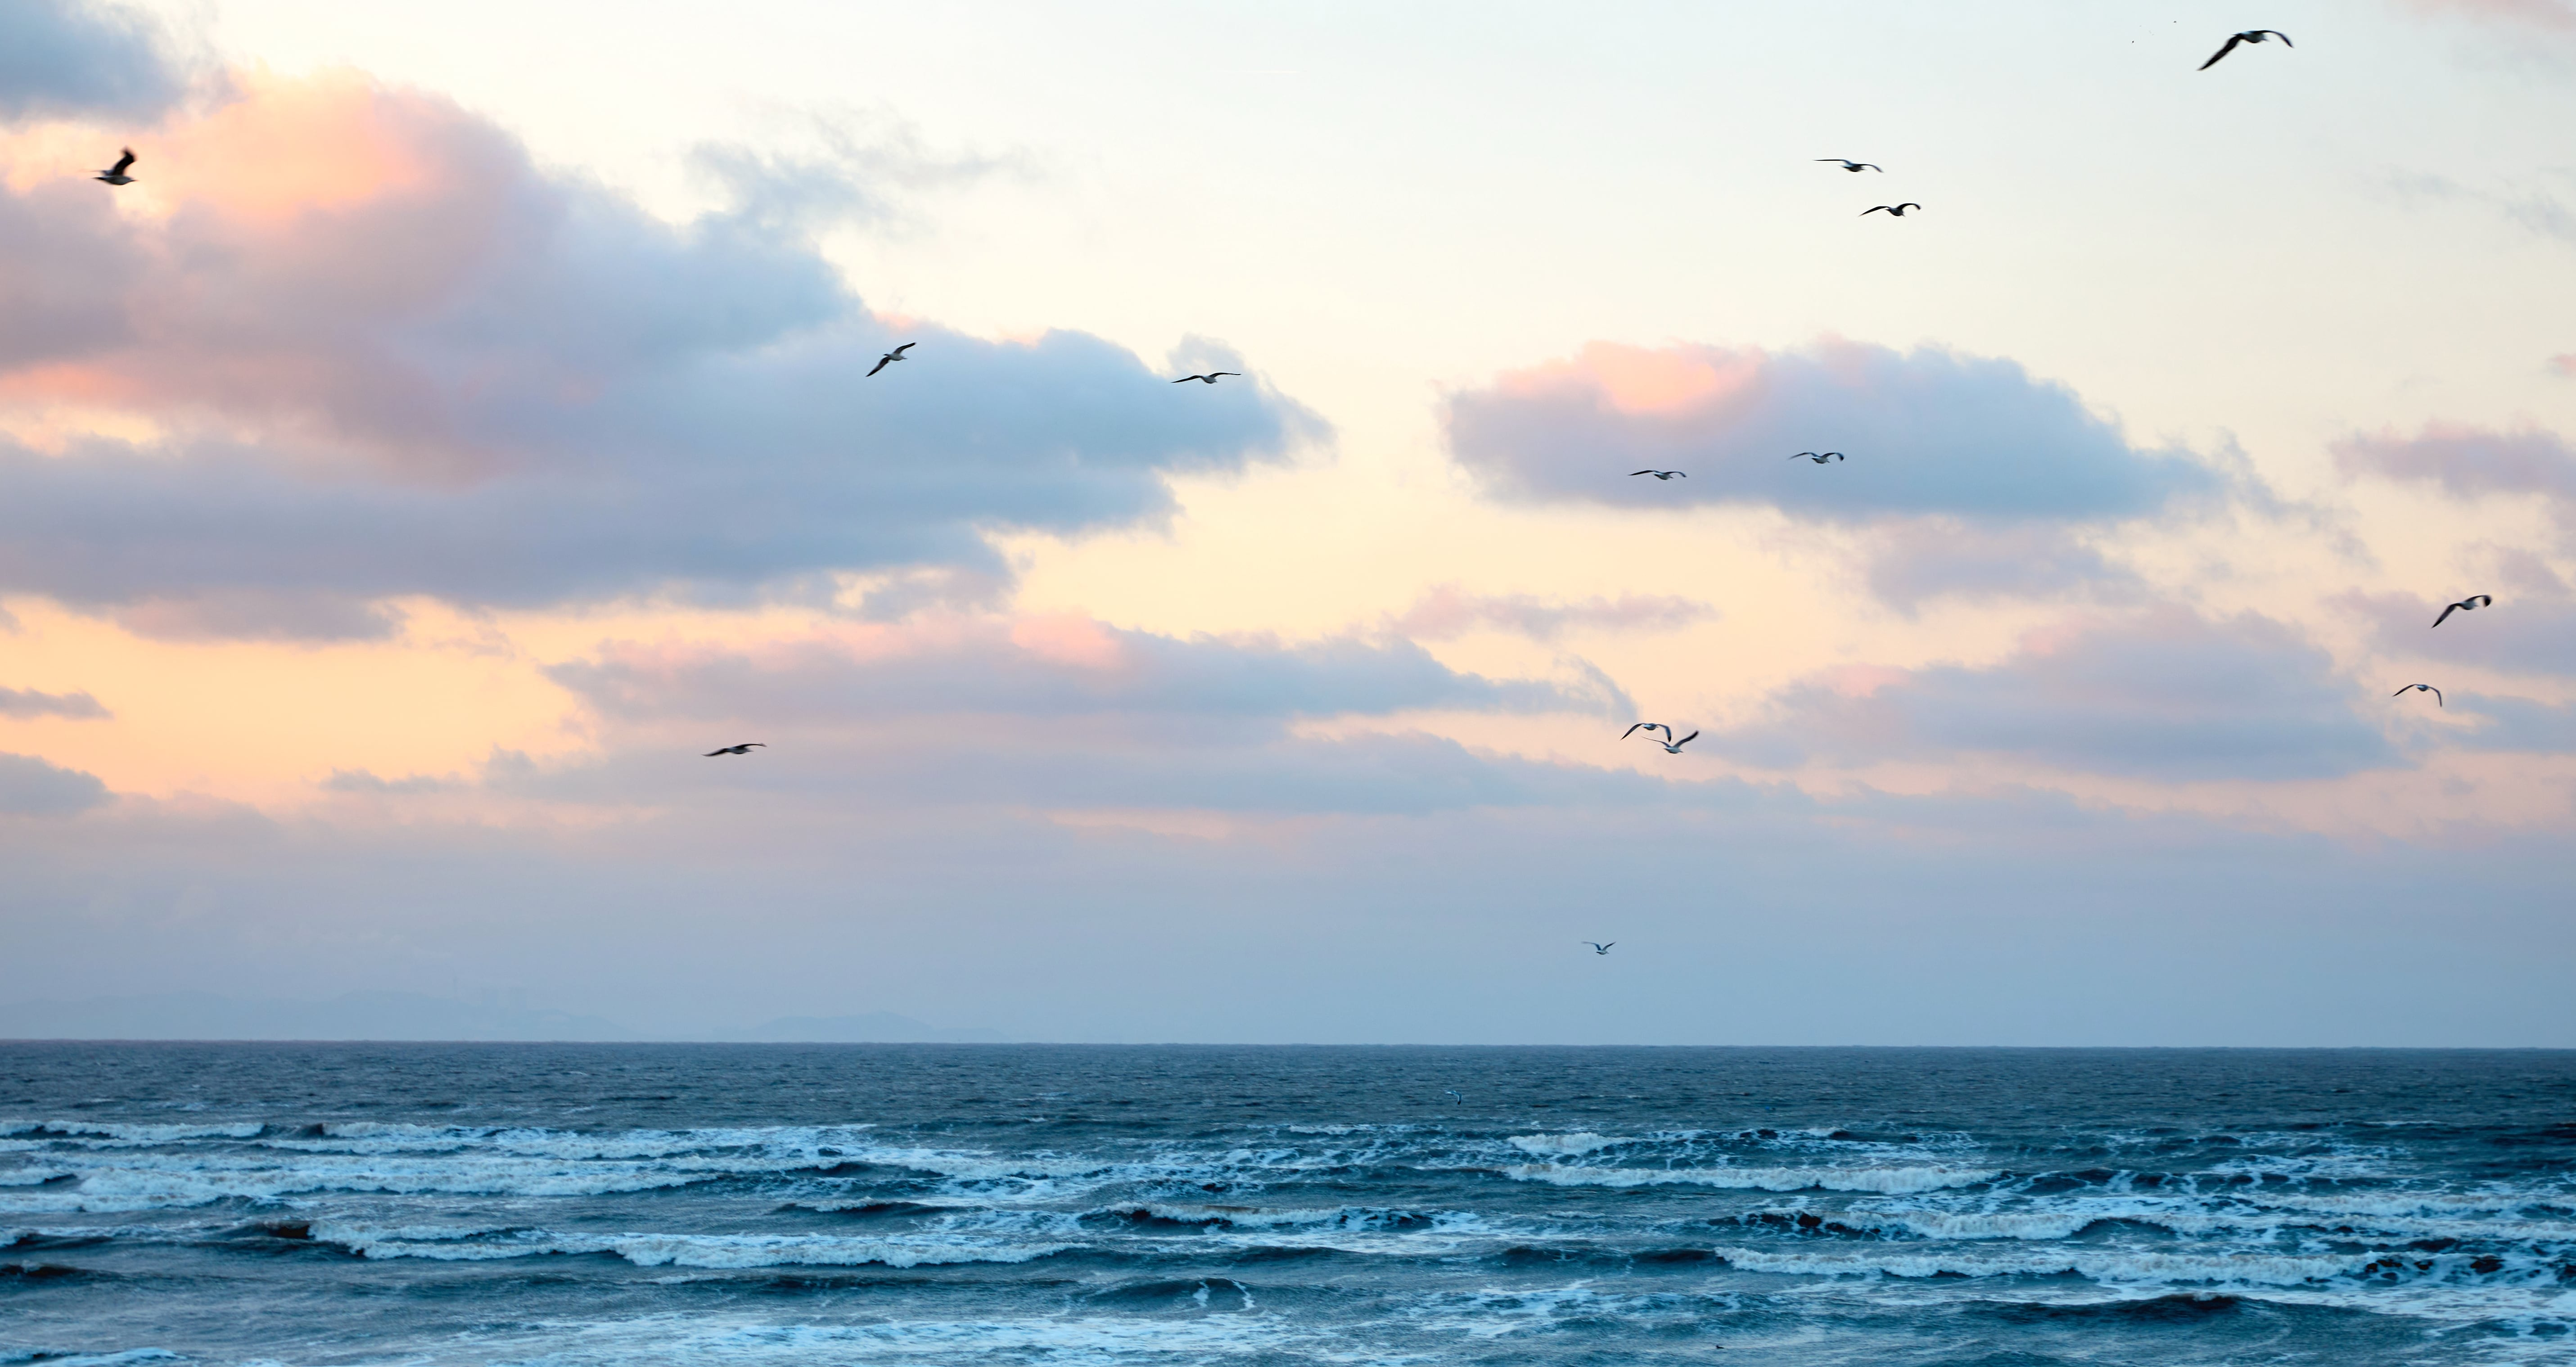
\includegraphics[width=0.75\linewidth]{figures/example2.jpg} % 图片路径
    \caption*{烟台的海、云朵与海鸥。} % 图片说明文字
    \caption{示例图片} % 图片标题
    \label{fig:example1} % 图片标签
\end{figure}
\vspace{-0.7em}  % 减少图片与正文间的间距


\section{多个图片}


该模板使用 \pkg{subcaption} 宏包来处理分图,呈现了如图 \ref{fig:multi-image-01} 、图 \ref{fig:multi-image-02} 所示的效果。

在图 \ref{fig:multi-image-01} 中,通过 \cs{subcaptionbox} 命令展示了两个独立的子图(图 \ref{fig:subfig-a-1} 和图 \ref{fig:subfig-b-1}),分别使用不同的标题,并被包含在总图标题“多个独立标题分图示例 01”中。

\begin{figure}[H]
    \centering
    \subcaptionbox{\label{fig:subfig-a-1}}{\includegraphics[width=0.35\linewidth]{example-image-a.pdf}}
    \subcaptionbox{\label{fig:subfig-b-1}}{\includegraphics[width=0.35\linewidth]{example-image-b.pdf}}
    \caption{多个独立标题分图示例 01}
    \label{fig:multi-image-01}
\end{figure}
\vspace{-0.7em}  % 减少图片与正文间的间距


\begin{figure}[H]
    \centering
    \subcaptionbox{分图 A1\label{fig:subfig-a-2-01}}{\includegraphics[width=0.17\linewidth]{example-image-a.pdf}}
    \subcaptionbox{分图 B1\label{fig:subfig-b-2-01}}{\includegraphics[width=0.17\linewidth]{example-image-b.pdf}}
    \subcaptionbox{分图 A2\label{fig:subfig-a-2-02}}{\includegraphics[width=0.17\linewidth]{example-image-a.pdf}}
    \subcaptionbox{分图 B2\label{fig:subfig-b-2-02}}{\includegraphics[width=0.17\linewidth]{example-image-b.pdf}}
    \caption{多个独立标题分图示例 02}
    \label{fig:multi-image-02}
\end{figure}
\vspace{-0.7em}  % 减少图片与正文间的间距


多个分图可以以多行的形式展示,使用的效果如图 \ref{fig:multi-image-03} 所示。

\begin{figure}[H]
    \centering
    \subcaptionbox{分图 A1\label{fig:subfig-a1-3}}{\includegraphics[width=0.25\linewidth]{example-image-a.pdf}}
    \subcaptionbox{分图 A2\label{fig:subfig-a2-3}}{\includegraphics[width=0.25\linewidth]{example-image-a.pdf}}
    \\
    \subcaptionbox{分图 B1\label{fig:subfig-b1-3}}{\includegraphics[width=0.25\linewidth]{example-image-b.pdf}}
    \subcaptionbox{分图 B2\label{fig:subfig-b2-3}}{\includegraphics[width=0.25\linewidth]{example-image-b.pdf}}
    \caption{多个独立标题分图示例 03}
    \label{fig:multi-image-03}
\end{figure}
\vspace{-0.7em}  % 减少图片与正文间的间距

两个图左右并排放置, 共用一个标题,使用的效果如图 \ref{fig:multi-image-04} 所示。

\begin{figure}[H]
\centering
    \includegraphics[width=0.25\linewidth]{example-image-a.pdf}
    \includegraphics[width=0.25\linewidth]{example-image-b.pdf}
    \caption{多个共用标题分图示例}
    \label{fig:multi-image-04}
\end{figure}
\vspace{-0.7em}  % 减少图片与正文间的间距

minipage 也可以实现排版并排插图, minipage 可以划分出虚拟的区块,每个区块中可以进行独立排版,使用的效果如图 \ref{fig:minipage-1} 和  \ref{fig:minipage-2} 所示。

\begin{figure}[H]
    \centering
    
    \begin{minipage}[H]{0.37\linewidth} % 第一个minipage
        \centering
        \includegraphics[width=0.49\linewidth]{example-image-a.pdf}
        \includegraphics[width=0.49\linewidth]{example-image-b.pdf}
        \\
        \includegraphics[width=0.49\linewidth]{example-image-a.pdf}
        \includegraphics[width=0.49\linewidth]{example-image-b.pdf}
        \caption{图 A1、图 B1、图 A2、图 B2}
        \label{fig:minipage-1}
    \end{minipage}
    \begin{minipage}[H]{0.37\linewidth} % 第二个minipage
        \centering
        \includegraphics[width=\linewidth]{example-image-c.pdf}
        \caption{图 C}
        \label{fig:minipage-2}
    \end{minipage}
    
\end{figure}
\vspace{-0.7em}  % 减少图片与正文间的间距


%%%%%%%%%%%%%%%%%%%%%%%%%%%%%%%%%%%%%%%%%%%%%%%%%%%%%%%%%%


\chapter{表格相关}


\section{普通三线表}

在 \LaTeX{} 中,表格的编辑相对较为复杂,推荐使用 Table Generator\footnote{Table Generator 网址:\url{https://www.tablesgenerator.com/}} 来生成表格。为使表格结构更加简洁通用,通常需要使用三线表。三线表是传统网格线表经过简化改造而来的,取消了斜线、竖线和横向分割线,表 \ref{tab:three-line} 是一个三线表的示例。

\begin{table}[H] % 表格位置固定
    \centering % 表格整体居中
    \caption{三线表示例} % 表格表题
    \label{tab:three-line} % 表格标签
    \renewcommand\arraystretch{0.85} % 定义表格行距
    \setlength{\tabcolsep}{12pt} % 定义列间宽度
    \begin{tabular}{ccc} % 表格列样式定义
        \toprule[1.5pt] % 顶线
        \textbf{列名1} & \textbf{列名2} & \textbf{列名3} \\ % 表头
        \midrule[0.8pt] % 栏目线
            Hunan & Hunan & Hunan \\ % 表体
            Yantai & Yantai & Yantai \\ % 表体
            Yantai & Yantai & Yantai \\ % 表体
        \bottomrule[1.5pt] % 底线
    \end{tabular}
\end{table}
\vspace{-0.5em}  % 减少表格与正文间的间距

表格如果有附注,尤其是需要在表格中进行标注时,可以使用 \pkg{threeparttable} 宏包。使用的效果如表 \ref{tab:three-line-with-note} 所示。

\begin{table}[H]
    \centering
    \caption{带附注的三线表示例}
    \label{tab:three-line-with-note}
    \renewcommand\arraystretch{0.85} % 定义表格行距
    \setlength{\tabcolsep}{15pt} % 定义列间宽度
    \begin{threeparttable}[c]
        \begin{tabular}{cc}
            \toprule[1.5pt]
            \textbf{山东省}  & \textbf{特色美食}\\
            \midrule[0.8pt]
            烟台           & 鲅鱼水饺、烟台焖子\\
            济南\tnote{a}  & 九转大肠\\
            青岛           & 青岛锅贴、青岛啤酒\\
            威海           & 手撕鲅鱼\\
            \bottomrule[1.5pt]
        \end{tabular}
        \begin{tablenotes}
            \item [a] {\zihao{5}众所周知,山东济南,中国青岛(狗头)}
        \end{tablenotes}
    \end{threeparttable}
\end{table}
\vspace{-0.9em}  % 减少表格与正文间的间距

\section{长表格}

如某个表需要转页接排,可以使用 longtable 宏包,需要在随后的各页上重复表的编号。
编号后跟表题(可省略)和“(续)”,置于表上方。续表均应重复表头。如表 \ref{tab:longTable} 所示。不过当一个张表内容过多时,建议将该表置于附录中。


\renewcommand\arraystretch{0.85} % 定义表格行距,注意命令的位置与普通表格不同
\begin{longtable}{cccccccc}
    \caption{跨页长表格} \\ % 换页前标题
    
    \toprule[1.5pt]
        \textbf{烟台} & \textbf{长沙} & \textbf{南昌} & \textbf{婺源} & \textbf{天津} & \textbf{上海} & \textbf{北京} & \textbf{青岛} \\ % 换页前表头
    \midrule[0.75pt]
    \endfirsthead
    
    \caption[]{跨页长表格(续)} \\ % 换页后标题
    \toprule[1.5pt]
        \textbf{烟台} & \textbf{长沙} & \textbf{南昌} & \textbf{婺源} & \textbf{天津} & \textbf{上海} & \textbf{北京} & \textbf{青岛} \\  % 换页后表头
    \midrule[0.75pt]
    \endhead
        \bottomrule[1.5pt]
        % \multicolumn{7}{r}{\textit{\zihao{5} \songti 接下页}} \\ 
    \endfoot 
    \bottomrule[1.5pt]
    \endlastfoot
    \label{tab:longTable}
        Row 01 & 01-01 & 01-02 & 01-03 & 01-04 & 01-05 & 01-06 & 01-07 \\
        Row 02 & 02-01 & 02-02 & 02-03 & 02-04 & 02-05 & 02-06 & 02-07 \\
        Row 03 & 03-01 & 03-02 & 03-03 & 03-04 & 03-05 & 03-06 & 03-07 \\
        Row 04 & 04-01 & 04-02 & 04-03 & 04-04 & 04-05 & 04-06 & 04-07 \\
        Row 05 & 05-01 & 05-02 & 05-03 & 05-04 & 05-05 & 05-06 & 05-07 \\
        Row 06 & 06-01 & 06-02 & 06-03 & 06-04 & 06-05 & 06-06 & 06-07 \\
        Row 07 & 07-01 & 07-02 & 07-03 & 07-04 & 07-05 & 07-06 & 07-07 \\
        Row 08 & 08-01 & 08-02 & 08-03 & 08-04 & 08-05 & 08-06 & 08-07 \\
        Row 09 & 09-01 & 09-02 & 09-03 & 09-04 & 09-05 & 09-06 & 09-07 \\
        Row 10 & 10-01 & 10-02 & 10-03 & 10-04 & 10-05 & 10-06 & 10-07 \\
        Row 11 & 11-01 & 11-02 & 11-03 & 11-04 & 11-05 & 11-06 & 11-07 \\
\end{longtable}
\vspace{-0.5em}  % 减少表格与正文间的间距




%%%%%%%%%%%%%%%%%%%%%%%%%%%%%%%%%%%%%%%%%%%%%%%%%%%%%%%%%%

\chapter{数学相关}

\section{数学符号}

中文论文的数学符号遵循 GB/T 3102.11—1993《物理科学和技术中使用的数学符号》标准\footnote{原 GB 3102.11—1993,自2017年3月23日起,该标准转为推荐性标准。},并参照 ISO 80000-2:2019。英文论文的数学符号采用 \TeX{} 默认的样式。

推荐使用 \href{http://mirrors.ctan.org/macros/latex/contrib/siunitx/siunitx.pdf}{\pkg{siunitx}} 宏包处理量和单位,以便方便地处理希腊字母以及数字与单位之间的空白。例如:
\SI{6.4e6}{m},
\SI{9}{\micro\meter},
\SI{30}{kg.m.s^{-1}},
\SI{20}{\degreeCelsius}。

表 \ref{tab:number} 展示了一些数字和单位的正确写法以及常见的错误写法。

\vspace{0.1em}
\begin{table}[H]
    \centering
    \caption{数字与单位示范}
    \label{tab:number}
    \renewcommand\arraystretch{0.85} % 定义表格行距
    \setlength{\tabcolsep}{15pt} % 定义列间宽度
    \begin{tabular}{@{}cc@{}}
        \toprule[1.5pt]
        \textbf{正确示例} & \textbf{错误示例} \\ 
        \midrule[0.8pt]
        \num{12345,67890} & 12345.67890 \\
        \num{.3e45} & 0.3 $\times$ 10\textsuperscript{45} \\
        \si{\kilo\gram\metre\per\square\second} & kg m s\textsuperscript{-2} \\
        \si{\square\volt\cubic\lumen\per\farad} & $V^{2}lm^{3}F^{-1}$ \\
        \SI[mode=text]{1.23}{J.mol^{-1}.K^{-1}} & 1.23J mol\textsuperscript{-1}K\textsuperscript{-1} \\
        \SI[per-mode=symbol]{1.99}[\$]{\per\kilogram} & \$ 1.99/kg \\
        \SI[per-mode=fraction]{1,345}{\coulomb\per\mole} & 1.345$\frac{C}{mol}$ \\ 
        \bottomrule[1.5pt]
    \end{tabular}
\end{table}
\vspace{-0.5em}  % 减少表格与正文间的间距


\section{数学公式}

在公式方面,作者用的最多的几种情况便是:有编号公式,无编号公式,多行公式按等号对齐等。需要注意的是,\textbf{默认情况下公式与上下文的间距可能过大}:
\begin{equation*}
    x_t = a_0 + a_1x_{t-1} + a_2x_{t-2} + \epsilon_t
\end{equation*}

因此如果有需要的话可以进行调整(详见该部分源码),调整效果如下:
\abovedisplayshortskip=3pt
\belowdisplayshortskip=3pt
\abovedisplayskip=3pt
\belowdisplayskip=3pt
\begin{equation*}
    x_t = a_0 + a_1x_{t-1} + a_2x_{t-2} + \epsilon_t
\end{equation*}

可以看到经过调整后,公式与上下文的间距缩小了,调整的值视情况而定即可。上面用到了equation*以生成不带编号的公式,而使用equation则可以生成自动编号(手动编号在这里就不演示了)的公式,如公式 \eqref{eq:example1}。
\begin{equation}
    x_t = a_0 + a_1x_{t-1} + a_2x_{t-2} + \epsilon_t
    \label{eq:example1}
\end{equation}

对于多行公式,如果不需要按等号对齐, 可以使用 \env{gather} 环境,如下:
\abovedisplayshortskip=3pt
\belowdisplayshortskip=4pt
\abovedisplayskip=3pt
\belowdisplayskip=4pt
\begin{gather*}%不会产生编号
max \ \ Cov(t_1,u_1) = Cov(Xw_1,Yv_1)\\
s.t.
\begin{cases}
  w_1^Tw_1 = \left \| w_1 \right \|^2 = 1  \\
  v_1^Tv_1 = \left \| v_1 \right \|^2 = 1  
\end{cases}
\end{gather*}

而如果需要多行公式尽可能在等号处对齐,可以使用 \env{align} 环境。
\abovedisplayshortskip=4pt
\belowdisplayshortskip=4pt
\abovedisplayskip=4pt
\belowdisplayskip=4pt
\begin{align}
Y &= t_1r_1^T + t_2r_2^T + \cdots + t_mr_m^T + Y_m \\
  &= (Xw_1^*)r_1^T + (Xw_2^*)r_2^T + \cdots + (Xw_m^*)r_m^T + Y_m \\
  &= X ({\textstyle \sum_{i=1}^{m}} w_ir_i^T) + Y_m
\end{align}

如果需要多个公式组在一起共用一个编号, 编号位于公式的居中位置,推荐使用 \env{aligned} 环境。使用效果如公式 \eqref{eq:example2} 所示。
\abovedisplayshortskip=4pt
\belowdisplayshortskip=4pt
\abovedisplayskip=4pt
\belowdisplayskip=4pt
\begin{equation}
\label{eq:example2}
\left\{
    \begin{aligned}
     & X = t_1p_1^T + t_2p_2^T + \cdots + t_mp_m^T \\
     & Y = t_1r_1^T + t_2r_2^T + \cdots + t_mr_m^T + Y_m
    \end{aligned}
\right.
\end{equation}




%%%%%%%%%%%%%%%%%%%%%%%%%%%%%%%%%%%%%%%%%%%%%%%%%%%%%%%%%%

\chapter{代码相关}

\section{伪代码}

伪代码(算法)环境可以使用 \pkg{algorithms} 宏包。算法 \ref{alg:decision_tree} 为演示的示例。

\begin{algorithm}
	\caption{Decision Tree Algorithm}
	\label{alg:decision_tree}
	\begin{algorithmic}[1]
		\STATE \textbf{Input:} Training dataset $D$, set of features $F$, current node $N$
		\STATE \textbf{Output:} Decision tree $DT$
		
		\IF{Stopping criteria are met for node $N$}
			\STATE Create a leaf node with the majority class in $D$
		\ELSE
			\STATE Select the best feature $f$ to split on
			\STATE Split $D$ into subsets $D_1$ and $D_2$ based on the value of feature $f$
			\STATE Create a decision node for $N$ with the split criterion $f$
			\STATE Recursively build the left subtree: $DT.left \leftarrow \text{BuildDecisionTree}(D_1, F, N_{\text{left}})$
			\STATE Recursively build the right subtree: $DT.right \leftarrow \text{BuildDecisionTree}(D_2, F, N_{\text{right}})$
		\ENDIF
		
		\RETURN $DT$
	\end{algorithmic}  
\end{algorithm}
\vspace{-0.5em}  % 减少表格与正文间的间距


\section{代码块}

代码环境可以使用 \pkg{lstlisting} 宏包。宏包可以自定义代码中关键字的高亮、代码块的边框、行号的样式等。代码 \ref{code:Python} 是一段 Pyhton 代码示例。


\vspace{-0.5em}
\begin{lstlisting}[label=code:Python, language=Python, caption=Python 代码示例]
sns.set(style='whitegrid', font_scale=1.3, rc={'figure.figsize': (20, 15), 'axes.edgecolor': '0.5'})
# Create a canvas with 15 subplots
fig, axes = plt.subplots(nrows=3, ncols=5, figsize=(26, 15), gridspec_kw={'wspace': 0.4, 'hspace': 0.4})
# colors
color = '#3498db'
# plot histgram
for i, ax in enumerate(axes.flatten()):
    if i < len(data.columns): 
        ax.hist(data.iloc[:, i], bins=20, color=color, edgecolor='black')
        ax.set_title(data.columns[i], fontsize=18)  
for i in range(len(data.columns), 3 * 5):
    axes.flatten()[i].axis('off')
\end{lstlisting}
\vspace{0.1em}



%%%%%%%%%%%%%%%%%%%%%%%%%%%%%%%%%%%%%%%%%%%%%%%%%%%%%%%%%%

\chapter{引用相关}

模板使用 \hologo{BibTeX} 处理引用参考文献。本章主要介绍 \hologo{BibTeX} 配合 \pkg{natbib} 宏包的主要使用方法\cite{mao2021correlation,tang2023lrbmat}。

\section{顺序编码制}

在顺序编码制下,默认的 \cs{cite\{\}} 命令同 \cs{citep\{\}} 一样,序号置于方括号中,引文页码会放在括号外。同一处引用的连续序号会自动用短横线连接。

\begin{table}[H]
  \centering
  \caption{顺序编码制中的对应关系}
      \begin{tabular}{l@{\quad$\Rightarrow$\quad}l}
      \verb|\cite{mao2021correlation}| & \cite{mao2021correlation}   \\
      \verb|\citet{mao2021correlation}| & \citet{mao2021correlation} \\
      \verb|\citep{mao2021correlation}| & \citep{mao2021correlation} \\
      \verb|\cite[42]{mao2021correlation}| & \cite[42]{mao2021correlation}  \\
      \verb|\cite{mao2021correlation,tang2023lrbmat}| & \cite{mao2021correlation,tang2023lrbmat} \\
      \end{tabular}
\end{table}
\vspace{-0.5em}  % 减少表格与正文间的间距

也可以通过 \cs{setcitestyle\{numbers\}} 设置引用样式为取消上标,将数字序号作为文字的一部分。

\setcitestyle{numbers} % 修改引用样式为取消上标格式

\begin{table}[H]
  \centering
  \caption{取消上标格式的顺序编码制中的对应关系}
      \begin{tabular}{l@{\quad$\Rightarrow$\quad}l}
      \verb|\cite{mao2021correlation}| & \cite{mao2021correlation} \\
      \verb|\citet{mao2021correlation}| & \citet{mao2021correlation} \\
      \verb|\citep{mao2021correlation}| & \citep{mao2021correlation} \\
      \verb|\cite[42]{mao2021correlation}| & \cite[42]{mao2021correlation}  \\
      \verb|\cite{mao2021correlation,tang2023lrbmat}| & \cite{mao2021correlation,tang2023lrbmat} \\
      \end{tabular}
\end{table}
\vspace{-0.7em}  % 减少表格与正文间的间距

\section{著者-出版年制}

可以通过 \cs{setcitestyle\{authoryear\}} 设置属性引用样式为著者-出版年制,其中 \cs{cite\{\}} 
跟 \cs{citet\{\}} 效果一样。

\setcitestyle{authoryear} % 修改引用样式为著者-出版年制

\begin{table}[H]
  \centering
  \caption{著者-出版年制中的对应关系}
      \begin{tabular}{l@{\quad$\Rightarrow$\quad}l}
      \verb|\cite{mao2021correlation}| & \cite{mao2021correlation} \\
      \verb|\citet{mao2021correlation}| & \citet{mao2021correlation} \\
      \verb|\citep{mao2021correlation}| & \citep{mao2021correlation} \\
      \verb|\cite[42]{mao2021correlation}| & \cite[42]{mao2021correlation}  \\
      \end{tabular}
\end{table}
\vspace{-0.5em}  % 减少表格与正文间的间距

\setcitestyle{super} % 修改引用样式为默认


%%%%%%%%%%%%%%%%%%%%%%%%  参考文献  %%%%%%%%%%%%%%%%%%%%%%%%

\begin{references}
    \bibliography{references.bib} % 指定.bib文件路径
\end{references}

%%%%%%%%%%%%%%%%%%%%%%%%%  附录  %%%%%%%%%%%%%%%%%%%%%%%%%%

\StartAppendix % 启用附录

\chapter{附录}

附录

%%%%%%%%%%%%%%%%%%%%%%%  正文后页眉  %%%%%%%%%%%%%%%%%%%%%%

% 页眉(关闭页眉务必将页眉类型设为empty)
\Header
    {common} % 页眉类型:common、publish、empty
    {1pt} % 上分隔线宽度
    {1pt} % 两线距离
    {0.5pt} % 下分割线宽度
    {} % 页眉左自定义内容(文本或图片)
    {
\includegraphics[width=0.25\textwidth]{figures/logos/HNU-title-EN.png}} % 页眉中自定义内容(文本或图片)
    {} % 页眉右自定义内容(文本或图片)

%============================================%

% 页脚(关闭页脚务必将页脚类型设为empty) 
\Footer
    {common} % 页脚类型:common、publish、empty
    {0pt} % 上分隔线宽度
    {0pt} % 两线距离
    {0pt} % 下分割线宽度
    {} % 页脚左自定义内容(文本或图片)
    {\thepage} % 页脚中自定义内容(文本或图片)
    {} % 页脚右自定义内容(文本或图片)

%============================================%

% 页数样式 参数:#1起始页数
% \setRomanPageNumber{1} % 设置罗马数字页码
% \setArabicPageNumber{1} % 设置阿拉伯数字页码

%%%%%%%%%%%%%%%%%%%%%%%%%  致谢  %%%%%%%%%%%%%%%%%%%%%%%%%

\StartAcknowledgements % 启用致谢

再次郑重感谢无私奉献的开源者们,开源了很多优秀的\LaTeX{}模板和详尽的示例文档,包括但不限于:
\href{https://github.com/tuna/thuthesis}{\textbf{ThuThesis}},
\href{http://aff.whu.edu.cn/huangzh/}{\textbf{武汉大学博士论文\LaTeX{}模板}},
\href{https://www.overleaf.com/latex/templates/dguttong-yong-lun-wen-slash-bao-gao-slash-zuo-ye-mo-ban-fei-guan-fang/gkymcyhwhjhj}{\textbf{DGUT通用论文模板}},
\href{https://www.overleaf.com/latex/templates/zhe-jiang-da-xue-ke-cheng-lun-wen-mo-ban/mjpzqvgsmdzn}{\textbf{浙江大学课程论文模板}},
\href{https://www.overleaf.com/latex/templates/scnu-my-article/jkbbvhnddtsw}{\textbf{SCNU-my-article}}和
\href{https://www.overleaf.com/latex/templates/shnu-thesis/wsykzrksspgn}{\textbf{SHNU-Thesis}}。
没有他们卓越的工作成果,该模板将很难完成。向每一位开源者致敬!

此外,还要感谢我的同学们。他们让我了解到了大家对于湖南大学自己的\LaTeX{}课程论文模板的需求\footnote{别的学校有的我们湖南大学也要有!(bushi)},并给予了我很多鼓励与支持。

希望该模板能对湖南大学的同学起到一些帮助,其他学校的同学亦可以把logo替换掉,进行更加个性化的设置。最后附上该项目GitHub链接:\url{????},如有错误或更改意见可以提交issue反馈。

\end{document}